\section{Baterías de ion-litio}

A finales del año 2019, año en el que se comenzó esta tesis, la Real Academia 
de Ciencias de Suecia le otorgó el Premio Nobel en Química a J. B. Goodenough, 
M. S. Whittingham y A. Yoshino por sus contribuciones al desarrollo de la batería 
de ion-litio \cite{nobel}. Esta batería recargable permitió los avances que se vieron en los 
teléfonos móviles y en las computadoras portátiles, entre otras aplicaciones.
Además, contribuye a lograr un mundo libre de combustibles fósiles ya que se utiliza en 
vehículos eléctricos y en almacenamientos estacionarios de energía para fuentes
renovables. Este galardón resaltó la importancia de muchos aspectos de la ciencia
moderna, como la investigación básica, la investigación la aplicada, la 
interdisciplina (JBG fue físico, MSW es un químico y AY un ingeniero), los 
desarrollos tecnológicos y los problemas concretos de las sociedades.
En la década del 1970, MSW desarrolló la primera batería utilizando un ánodo de
litio metálico y un cátodo de disulfuro de titanio \cite{whittingham1976}. En 
1980, JBG duplicó el voltaje original de dicha batería al introducir un cátodo 
de óxido de cobalto \cite{mizushima1980}.
La desventaja de ambas se encontraba en el ánodo de litio metálico, que en los 
ciclos de carga y descarga se deposita preferentemente en sitios donde ya se 
ha depositado, dando lugar a estructuras ramificadas, llamadas dendritas, que 
pueden cortocircuitar la celda y llevar a la explosión de la misma. En 1985,
AY reemplazó este material por uno carbonoso que incorpora los iones de litio
durante la carga y la descarga, disminuyendo los riesgos mencionados. Basándose
en este desarrollo, Sony comenzó a comercializar baterías de ion-litio en 1991.
La densidad de energía de estas baterías rondaba los 80 Wh/kg, en la actualidad
WeLion comercializa para los EVs de Nio una batería de ion-litio con una 
densidad de energía de 360 Wh/kg \cite{li2023700}. En la Figura \ref{fig:whkg} se muestra la 
evolución de la densidad de energía en baterías de ion-litio comercializadas 
en los últimos 30 años. La importancia de esta característica para los EVs 
radica en la relación autonomía/peso. Además de este, existen otros parámetros 
que tienen que tenerse en cuenta, como la cantidad de ciclos que se pueden 
realizar, el tiempo que toma realizar la carga y el 
precio de producción.
\begin{figure}[h!]
    \centering
    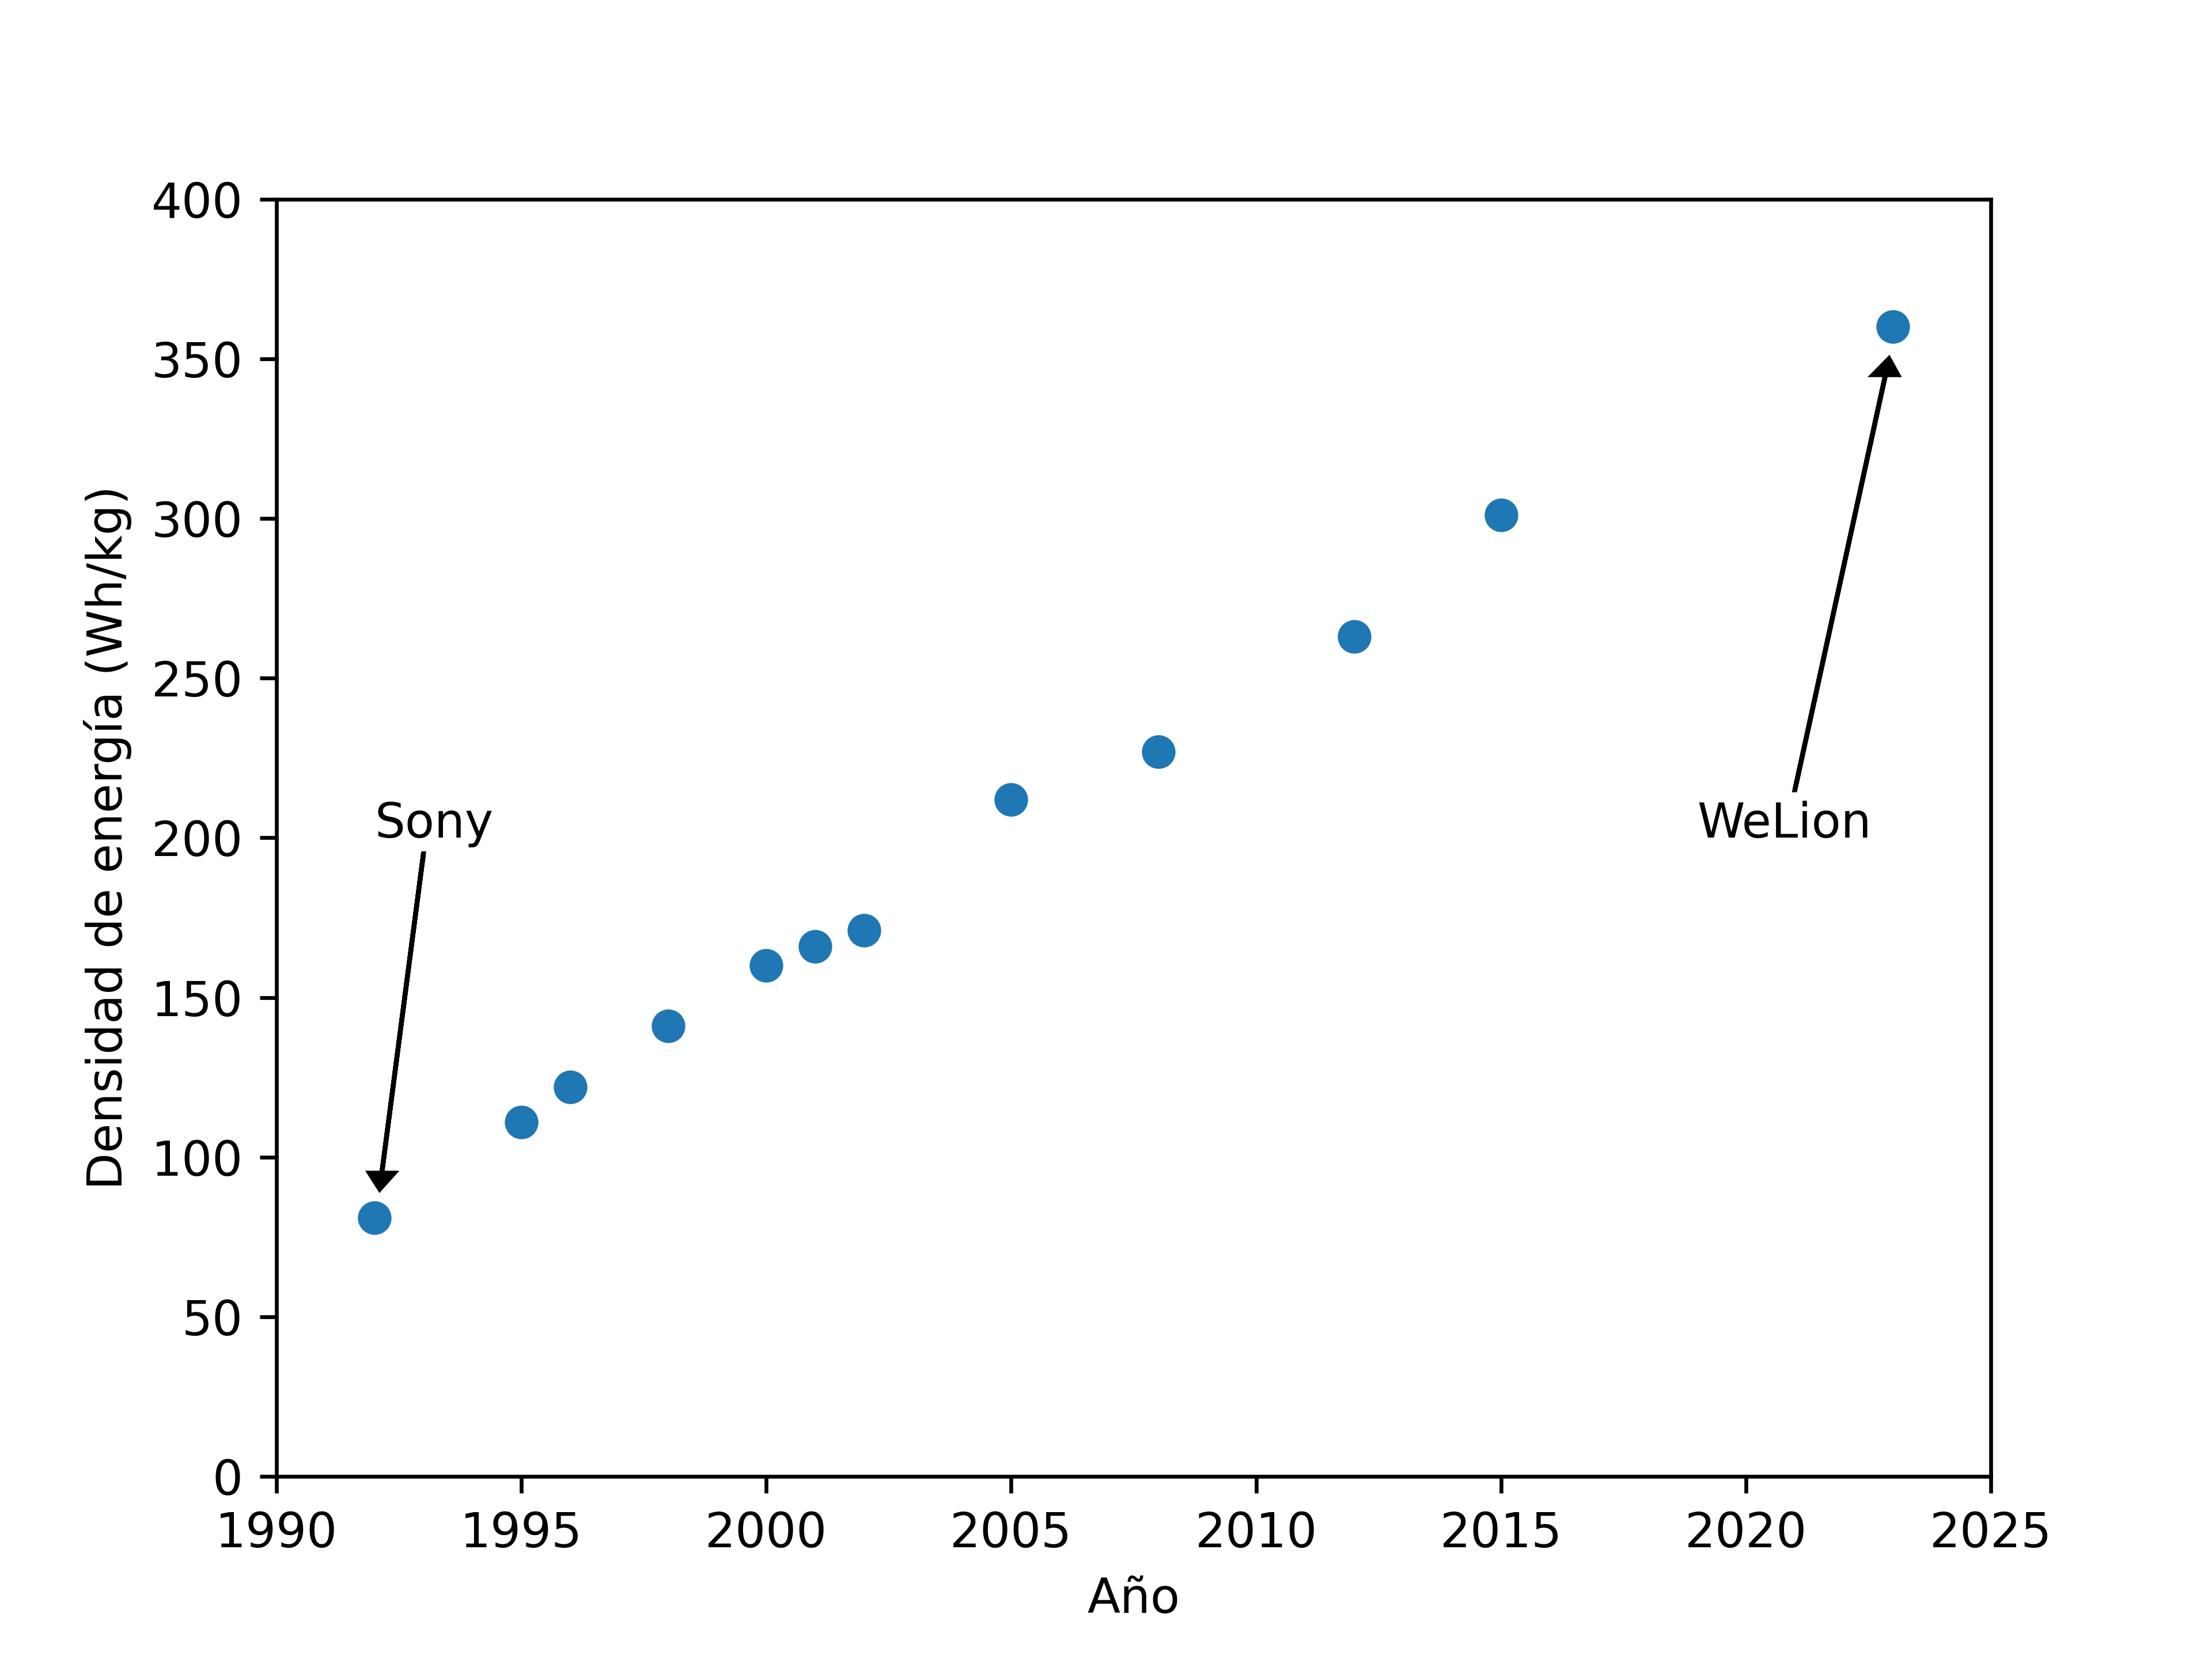
\includegraphics[width=.8\textwidth]{Introduccion/baterias/whkg.png}
    \caption{Aumento en la densidad de energía en baterías de ion-litio comercializadas
    en los últimos 30 años. Figura adaptada de \cite{li2023700}.}
    \label{fig:whkg}
\end{figure}

Las baterías de ion-litio (LIBs, de sus siglas en inglés \textit{Lithium-Ion 
Batteries}) admiten una gran cantidad de recargas y las mismas están compuestas 
por celdas electroquímicas conectadas entre sí. Estas celdas electroquímicas son unidades 
fundamentales que permiten transformar la energía química almacenada en energía
eléctrica mediante una reacción redox (reducción-oxidación), en la cual uno de los 
componentes pierde electrones (se oxida) y el otro gana electrones (se reduce).
En la Figura \ref{fig:esquema-bateria} se muestra un esquema general con el 
funcionamiento que presenta una celda electroquímica de ion-litio y se destacan 
las componentes más relevantes: los electrodos positivo (cátodo) y negativo (ánodo) 
donde ocurren las reacciones redox en la carga/descarga de la celda, el electrolito 
por el cual difunden los iones de litio y el separador, que es un material 
poroso permeable al electrolito que permite que los iones circulen dentro del electrolito.
Durante la descarga, la reacción redox es espontánea y 
provoca la difusión de iones de litio por el electrolito desde el ánodo hacia el 
cátodo, junto con una corriente eléctrica en un circuito externo (flechas rojas). 
Durante la carga se debe aplicar una corriente eléctrica externa para tener la 
reacción inversa (flechas verdes).
Por el principio de electroneutralidad, la entrada (salida) a cada electrodo de una cierta cantidad de iones de litio, implica recíprocamente la entrada (salida) de un número equivalente de electrones.
\begin{figure}[h!]
    \centering
    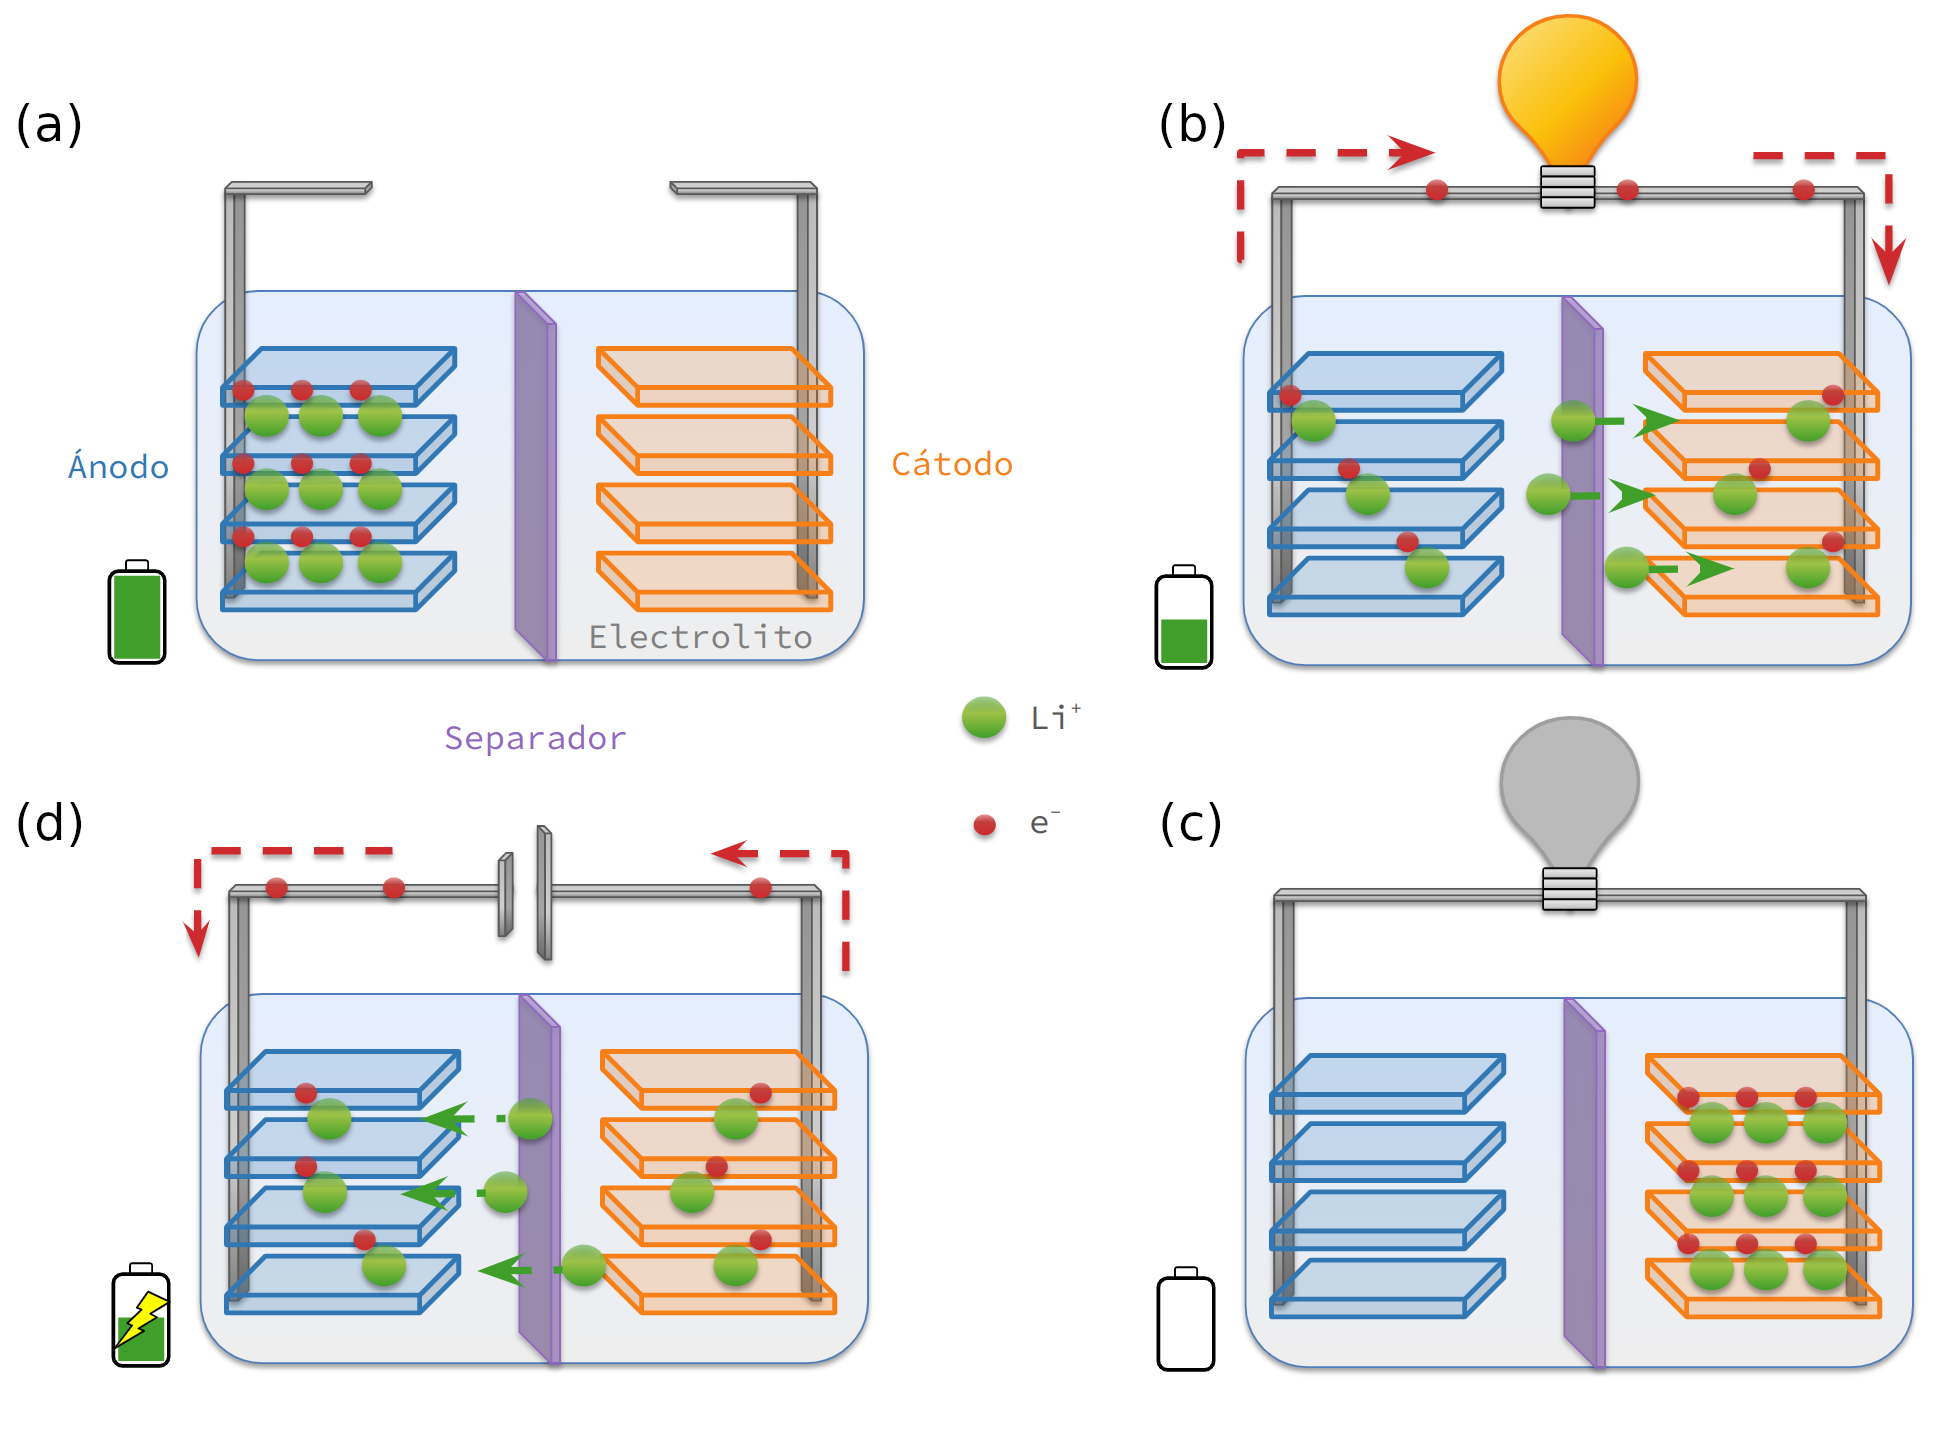
\includegraphics[width=.8\textwidth]{Introduccion/baterias/esquema_bateria.png}
    \caption{Esquema de las componentes y el funcionamiento de una batería de 
    ion-litio.}
    \label{fig:esquema-bateria}
\end{figure}

La tendencia obtenida en el aumento de densidad de energía, ya observada de la 
Figura \ref{fig:whkg}, fue posible gracias a una mejor ingeniería en la celda. 
Los próximos grandes desafíos en el área de estudio aparecen en el desarrollo de 
nuevos materiales en cada una de sus componentes en las baterías introducidas.
Por ejemplo, la ya mencionada batería de WeLion introduce materiales distintos 
de aquellos implementados originalmente por Sony. A continuación se mencionan
algunas variantes a las distintas partes de las baterías presentadas en la
Figura \ref{fig:esquema-bateria} que se encuentran en etapas de investigación 
y algunas de ellas ya comercializadas.

Con respecto a los cátodos, idealmente deben ser estables a temperatura ambiente,
tener un voltaje y una capacidad específica alta. Además, se busca que no sean 
tóxicos y que sean amigables con el medioambiente. Los cátodos más utilizados 
suelen ser metales de transición, como el ya mencionado óxido de cobalto 
(LiCoO$_2$ o LCO), que posee una capacidad teórica relativamente alta de 274 mAhg$^{-1}$ y un buen desempeño en su ciclabilidad, pero es un
material caro y tóxico \cite{akhilash2021}. Una alternativa que aparece frente
al mismo es el LiNiO$_2$ (LNO), que es isoestructural al LCO, posee una
capacidad teórica similar de 273 mAhg$^{-1}$ y tiene un menor costo. Sin embargo, es
difícil de sintetizar y se ha observado la formación de una fase 
electroquímicamente inactiva cuando la concentración de litio alcanza el 50\% 
\cite{bianchini2019}. Otra de las variantes propuestas al LCO es la espinela
LiMnO$_2$ (LMO), que presenta un voltaje alto, cercano a los 4 V vs Li/Li$^+$,
es más barato que el LCO y no es tóxico. Sin embargo, el LMO presenta una 
pérdida considerable de la capacidad con los ciclos \cite{bhandari2016}. Basándose en estos 
tres metales de transición se han desarrollado compuesto de intercalación con 
la fórmula general Li(Ni$_{1-x-y}$Co$_x$Mn$_y$)O$_2$ (NMC). Para conseguir un 
material catódico viable, existen relaciones de compromiso entre las proporciones de cada uno de 
los metales según los aspectos que se deseen: alta capacidad (más níquel), 
mejor estabilidad de ciclado (más cobalto) o seguridad/costo (más manganeso). 
También se han investigado los cátodos L(Ni$_{0.5}$Mn$_{1.5}$)O$_2$ (NMO) debido
a su densidad de energía similar a la del LCO pero con una reducción en los costos.
Además, se han obtenido capacidades cercanas a los 180 mAhg$^{-1}$ a una C-rate de 6 C.
Otra de las opciones es el dopaje de LiNiO$_2$ con cationes de cobalto y aluminio, 
Li(Ni$_{1-x-y}$Co$_x$Al$_y$)O$_2$ (NCA), que en la composición 
Li(Ni$_{0.8}$Co$_{0.15}$Al$_{0.05}$)O$_2$ \cite{chen2004} es comercializada 
dentro de algunos de los modelos de EVs de Tesla, ya que posee una capacidad alta ($\sim$ 200 mAhg$^{-1}$) y una gran vida útil comparada a la del LCO. Por otro lado, la olivina 
LiFePO$_4$ (LFP) fue introducida como material catódico a fines de la década 
de 1990 por el grupo de Goodenough \cite{padhi1997}, donde encontraron capacidades
menores a los 120 mAhg$^{-1}$, pero ganó interés debido a su estabilidad térmica, su bajo costo y a la 
naturaleza ambiental benigna del fosfato de hierro. Los problemas asociados al LFP son la
conductividad eléctrica y la difusividad del litio bajas, sin embargo, debido
a sus ventajas ya ha sido exitosamente comercializado, por ejemplo en los EVs 
TITO fabricados en la provincia de San Luis.

Los electrolitos son sistemas conformados por una mezcla de disolventes, una 
sal y aditivos. Las soluciones electrolíticas que se utilizan en las LIBs actuales 
consisten disolventes de carbonato de etileno (EC) y carbonatos lineales, como
el carbonato de etilo y metilo (EMC) o el carbonato de dimetilo (DMC), combinados 
con LiPF$_6$ como sal de litio. Los aditivos que se utilizan en las soluciones 
comerciales no suelen divulgarse ~\cite{schipper2016}. Algunas de las 
investigaciones que se llevan a cabo en la actualidad incluyen solventes de
baja viscosidad ~\cite{logan2020}, mejoras en su seguridad ~\cite{wang2019} 
y en electrolitos de estado sólido ~\cite{zheng2018}.

En lo que respecta al ánodo, en 1990 el grupo de Jeff Dahn \cite{fong1990} propuso 
la utilización de grafito, que ha dominado el mercado de las baterías debido a
la estabilidad de los mismos, su expansión volumétrica leve del 10\% durante 
la (de)intercalación de litio, su alta conductividad y buena eficiencia; además, 
es un material abundante y no es tóxico. Otro material anódico de intercalación 
es el titanato de litio Li$_4$Ti$_5$O$_{12}$ (LTO) que posee la ventaja de 
no sufrir cambios estructurales durante el proceso de (de)intercalación de litio, 
pero su potencial de operación es relativamente alto y por lo tanto su densidad energética es baja comparada a otros ánodos. Otro proceso que
puede darse en los ánodos durante su carga es la aleación de los iones de litio 
con algún otro elemento químico. Dentro de estos materiales se encuentran el silicio y el estaño
que poseen capacidades teóricas de 3579 mAhg$^{-1}$ y 960 mAhg$^{-1}$, 
respectivamente. Ambos materiales además cuentan con las ventajas de ser baratos,
abundantes y amigables con el medio ambiente. Sin embargo, ambos presentan un 
cambio de volumen durante la litiación y la delitiación que ronda el 300\% y 
lleva asociado pérdidas en la capacidad irreversibles desde el primer ciclo.
Algunas de las causantes de estas desventajas son: la pulverización de 
partículas que provoca la desconexión con el colector de carga, la formación de 
una SEI (\textit{solid-electrolyte interface}) renovada en cada ciclo y la 
retención de iones de litio en las aleaciones debido a la cinética lenta o a la
formación de aleaciones altamente estables. Para reducir estos problemas se 
han desarrollado y se continúan estudiando distintas estrategias, entre ellas,
por ejemplo, la utilización de nanoestructuras, matrices para disminuir la 
tensión y construcción de compartimentos para acomodar la expansión 
volumétrica \cite{zuo2016}. Sin embargo, para algunas de ellas son necesarios pasos 
experimentales complicados que requieren mucho tiempo, son costosos y difíciles
de escalar con fines de producción comercial.

\todo{
Otros materiales que experimentan procesos distintos también han llamado la 
atención de la comunidad científica \cite{nitta2015}; entre ellos destacan el 
azufre, debido a su capacidad teórica de 1675 mAhg$^{-1}$, su bajo costo y su 
abundancia en la tierra. Otro caso llamativo es el del oxígeno para las baterías
de litio/aire, que presenta distintos obstáculos tecnológicos al ser un gas.
}

En la Figura \ref{fig:scopus} se muestra el incremento en las últimas dos décadas
de los artículos científicos publicados en el área de las baterías de litio y, en 
particular, de las dos ramas estudiadas en esta tesis: la carga rápida y los 
ánodos de Si. En dicha figura se presentan datos extraídos de la base de datos 
Scopus \cite{SCOPUS}, acerca del número de publicaciones anuales normalizado con respecto 
al número de publicaciones en el año 2003, año en el que hubo 710 publicaciones 
en baterías de litio, 32 sobre ánodos de Si y 0 sobre carga rápida, por lo que 
se normalizó en este caso a la única publicación del 2004 en el tema.
\begin{figure}[h!]
    \centering
    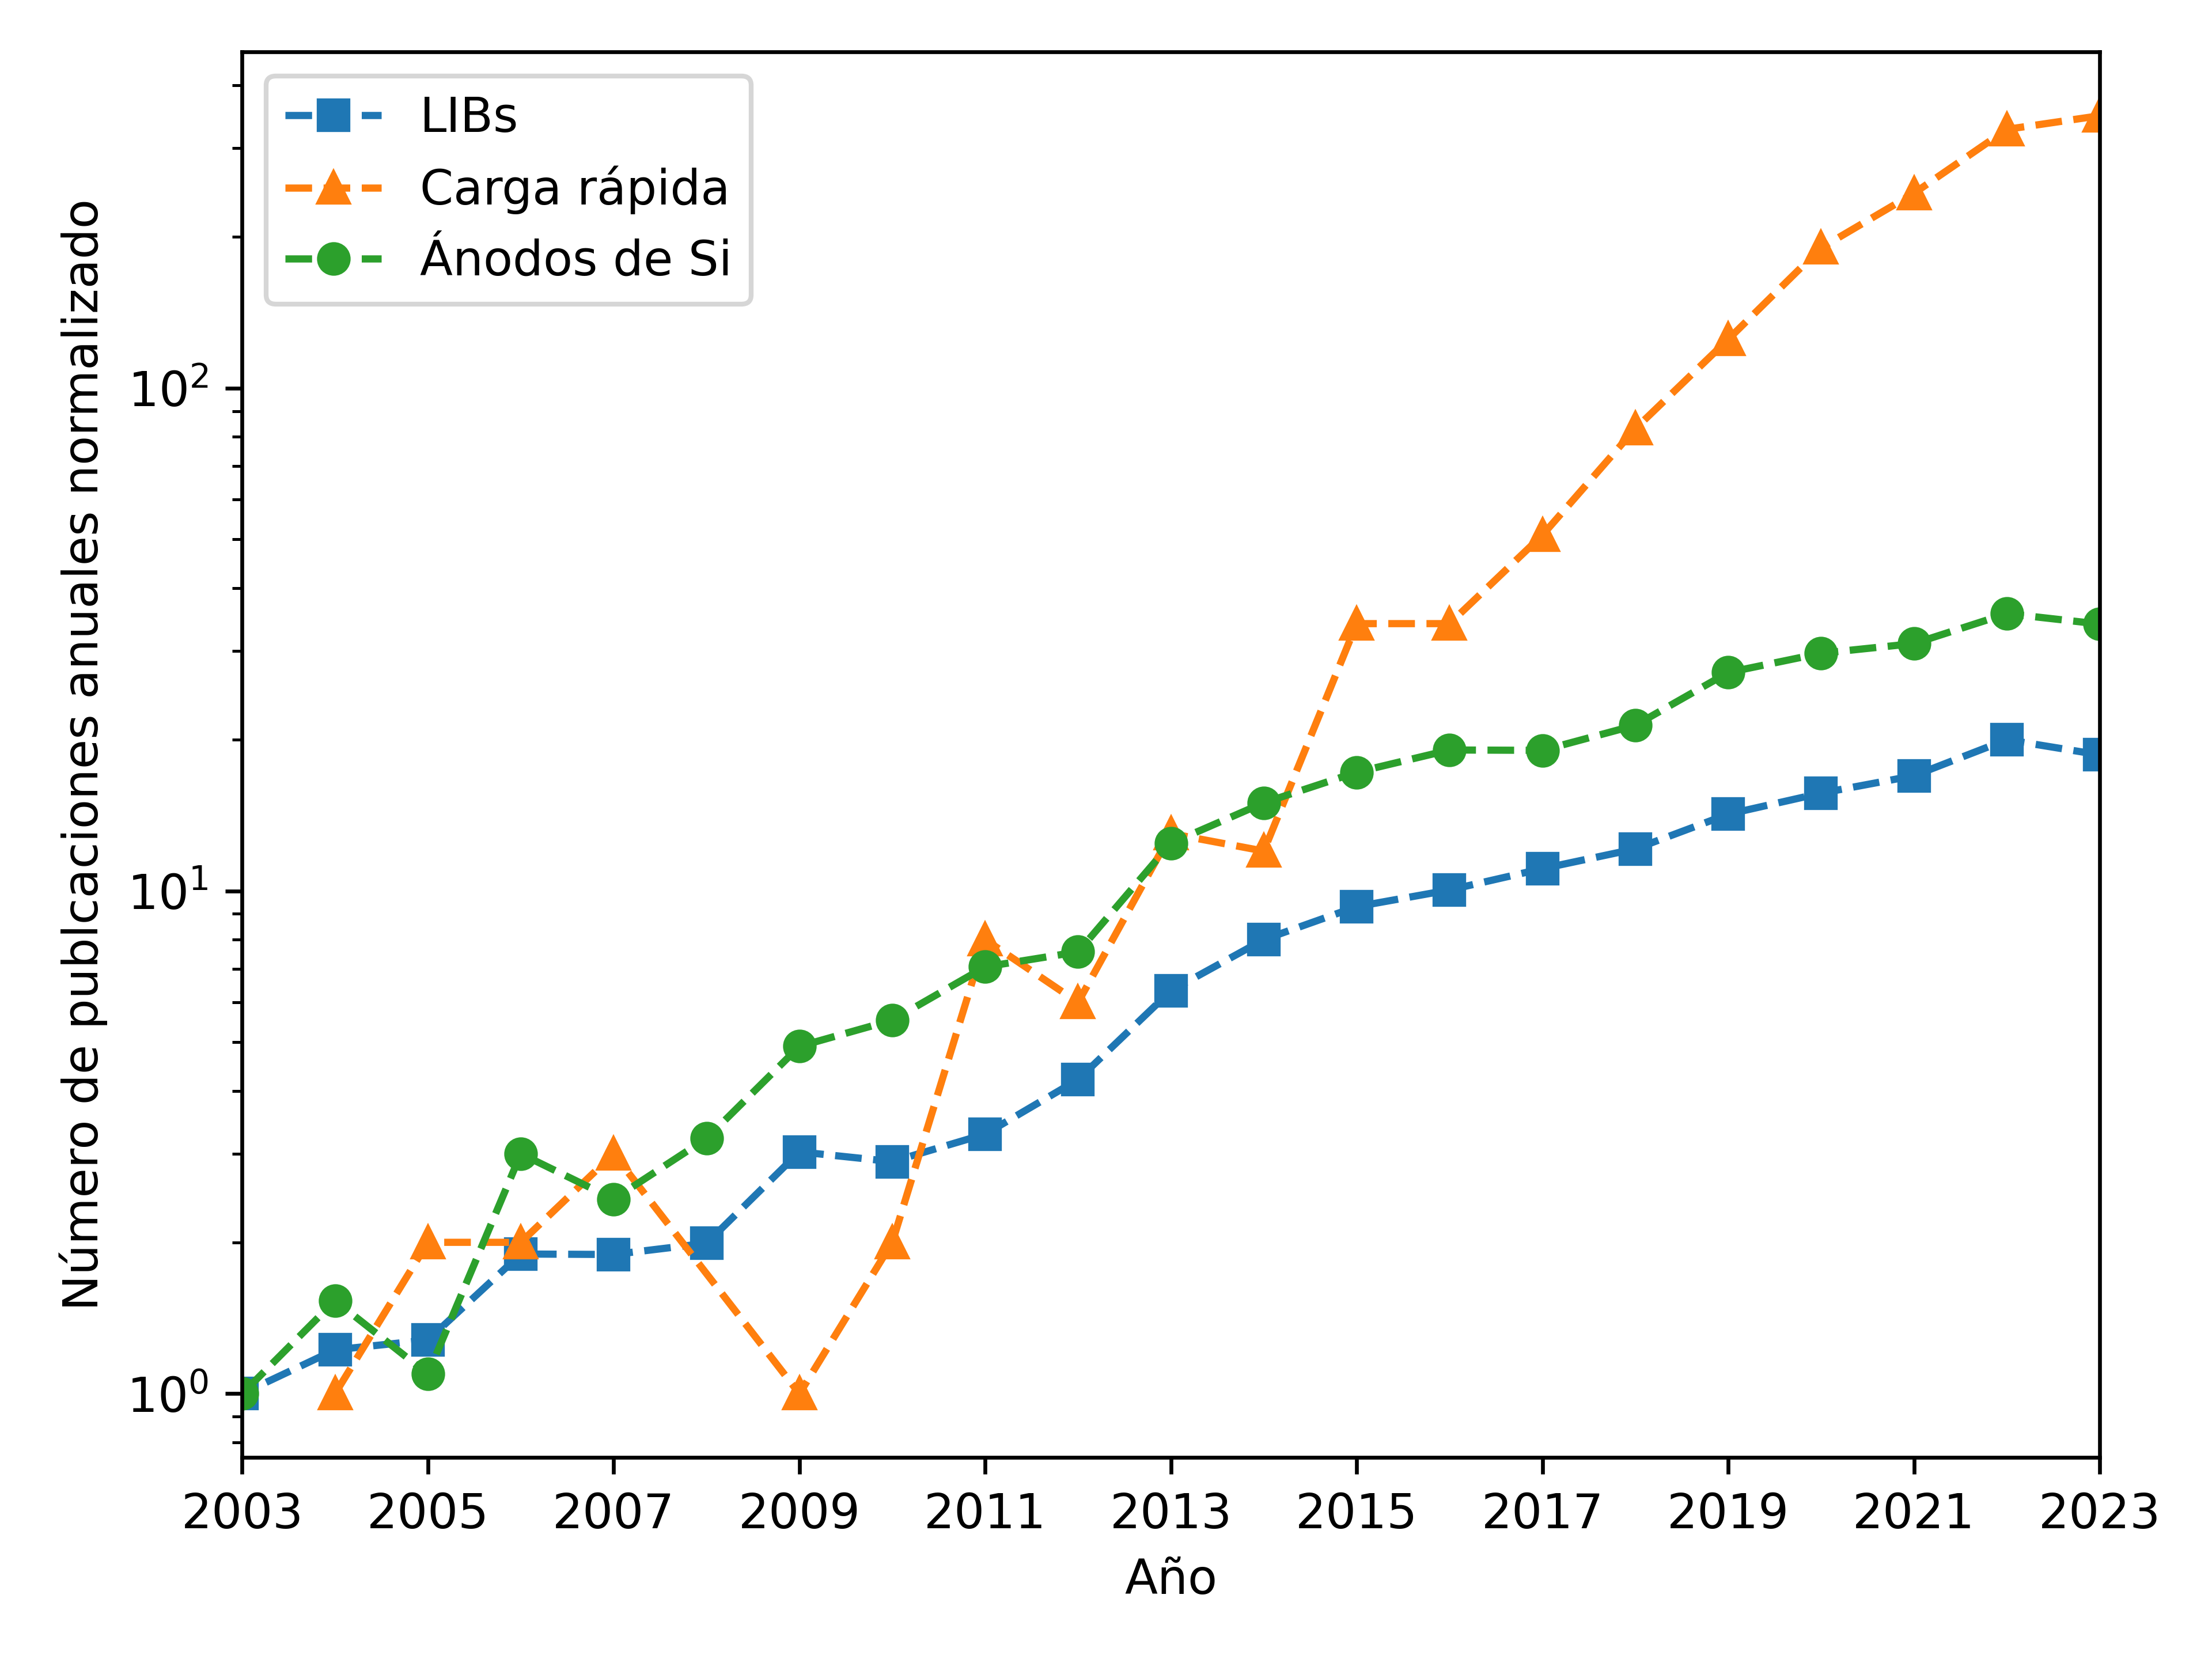
\includegraphics[width=.8\textwidth]{Introduccion/baterias/scopus.png}
    \caption{Número de publicaciones anuales normalizado con respecto al año 2003. 
    Las consultas realizadas en Scopus \cite{SCOPUS} incluyen: 
    \texttt{lithium AND battery} (LIBs, en azul), \texttt{lithium AND battery AND 
    fast-charging} (Carga rápida, en naranja) y \texttt{lithium AND battery AND 
    silicon anodes} (Ánodos de Si, en verde).}
    \label{fig:scopus}
\end{figure}
La normalización y la escala logarítmica en la Figura \ref{fig:scopus} permiten
observar cualitativamente que la pendiente de crecimiento de publicaciones 
relacionadas a la carga rápida de baterías de litio es considerablemente mayor que 
de las otras dos. Además, los ánodos de Si se encuentran dentro de lo que sería
el crecimiento promedio del área de las baterías de litio. Un análisis 
cuantitativo permite determinar que en la última década el aumento de porcentaje
anual de publicaciones promedio fue del 15\% y 16\% para las baterías de litio 
y para los ánodos de silicio, respectivamente, mientras que para la carga rápida 
este porcentaje promedio asciende al 52\%. Este análisis de datos demuestra la relevancia
que la comunidad científica le da a los temas estudiados en esta tesis.
